\subsubsection{Yee Cell and Leapfrog Method}

According to ref.~\cite{yee} Eq.~\ref{eq:maxwell} is discretized with $t=q\Delta_t$ and $x=m\Delta_x$ where $q,m\in\left\{\dots,-1,-\frac{1}{2},0,\frac{1}{2},1,\dots\right\}$ and $\Delta_x, \Delta_t$ being the division of our space and time grid.

Taking equation~\ref{eq:maxwell} and using the time steps $q+\frac{1}{2}$ and $q-\frac{1}{2}$ and the partition steps $m+1$ and $m$ this gives

\begin{equation}
  \mu\frac{H_y\left[\left(q+\frac{1}{2}\right)\Delta_t, (m+\frac{1}{2})\Delta_x\right]-H_y\left[\left(q-\frac{1}{2}\right)\Delta_t, (m+\frac{1}{2})\Delta_x\right]}{\Delta_t}=\frac{E_z\left[q\Delta_t, (m+1)\Delta_x)-E_z(q\Delta_t, m\Delta_x)\right]}{\Delta_x}.
\end{equation}

Solving for future $H_y$ yields

\begin{multline}
  H_y\left[\left(q+\frac{1}{2}\right)\Delta_t, \left(m+\frac{1}{2}\right)\Delta_x\right]=H_y\left[\left(q-\frac{1}{2}\right)\Delta_t, \left(m+\frac{1}{2}\right)\Delta_x\right] +\\
  \underbrace{\frac{\Delta_t}{\mu\Delta_x}\left(E_z\left[q\Delta_t, (m+1)\Delta_x\right]-E_z\left[q\Delta_t, m\Delta_x\right]\right)}_\text{update function for $H_y$}.
\end{multline}

This means the value of the magnetic field at a given point $(m+1/2)\Delta_x$ can be calculated from it's last value and the surrounding electric fields at a prior time. The difference between $H_y((q+\frac{1}{2})\Delta_t)$ and $H_y((q-\frac{1}{2})\Delta_t)$ is called the update function.

Likewise these calculations can be done for $E_z$ to get an update function to calculate the next value of $E_z$ from it's old value and the surrounding two $H_y$ values.

\begin{figure}[!h]
  \centering
  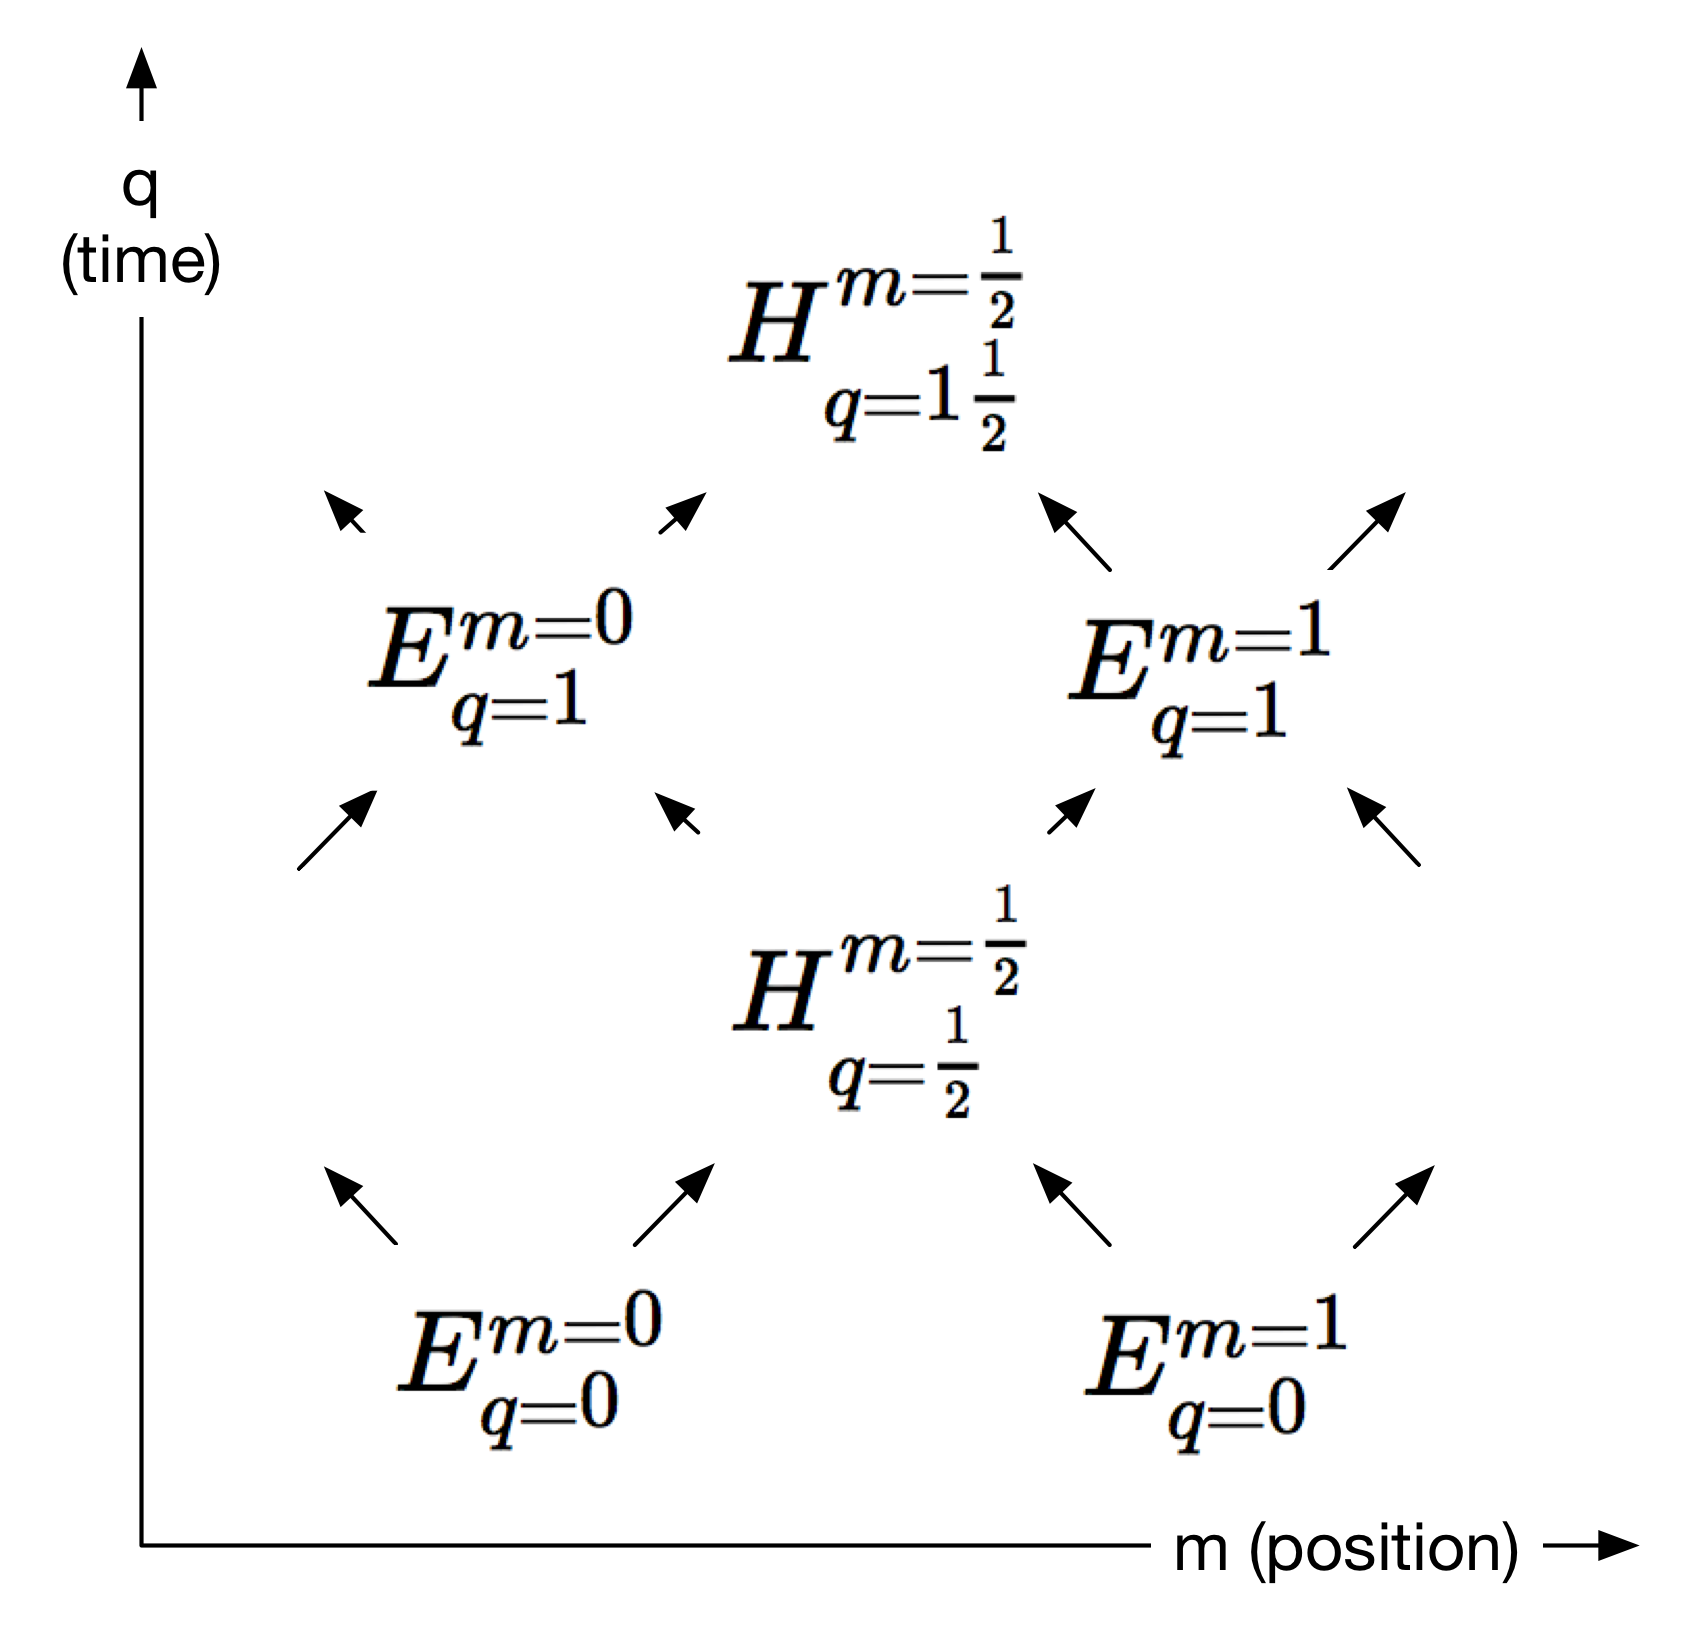
\includegraphics[width=0.5\textwidth]{./images/space-time-cell.png}
  \caption{Each value of $\mathbf{E}$ at a specific time can be calculated by the former value at the same position in space one time step before and the surrounding values of $\mathbf{H}$ half a timestep before. Following this algorithm the diagram is built from bottom to top line by line which is the reason this method is called leapfrog method. \note{use 3/2 instead of  1 1/2}}
  \label{fig:leapfrog}
\end{figure}

To get the electric field of any given system at a specific time this algorithm calculates $E_z$ and $H_y$ with $q$ starting at 0 and increasing by $\frac{1}{2}$ until the required time $t = q\Delta_t$ is reached, as schematically shown in figure~\ref{fig:leapfrog}. The only required input is the initial field of $E_z$ at $q = 0$. Because this method calculates $E$ and $H$ in turns it is also called the "leap frog method".

To account for different materials within the system, $\mu$ can be replaced by a location or even time dependent $\mu(t, x)$.

\begin{figure}[!h]
  \centering
  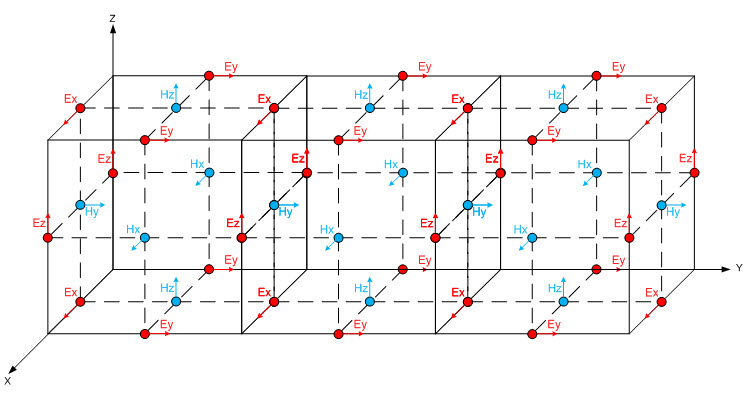
\includegraphics[width=0.8\textwidth]{./images/yeecell.jpg}
  \caption{To visualize the different points that are calculated during the process for three dimensions there is the so called Yee Cell that is formed by taking the points for $\mathbf{E}$ at $q=0$ and $\mathbf{H}$ at $q=\frac{1}{2}$. Each value for $\mathbf{H}$ can be calculated by its surrounding values of $\mathbf{E}$ at the time step $q-\frac{1}{2}$.}
\end{figure}

\note{add paragraph about step to 3D and yee cell}
